\chapter{Un tour de C}
\label{cha:tour}
\thispagestyle{empty}

%% Calculate how old C is...
\newcount\cdifference\cdifference=\the\year\advance\cdifference by -1970

C is al een oude taal. De taal is rond 1970 ontworpen door Dennis Ritchie\footnote{Dennis MacAlister Ritchie (1941 -- 2011). Hij was de ontwerper van de programmeertaal C en was een van de ontwerpers van Unix. Bekende afgeleiden van Unix zijn Linux en FreeBSD.} en is dus al zo'n \the\cdifference\ jaar oud. Hij was bezig met het schrijven van een besturingssysteem (Engels: operating system)\footnote{Een besturingssysteem is een programma dat draait op een computer en zorgt voor het beschikbaar stellen van \textsl{resources} aan de gebruiker (lees: programma's). Zo zorgt een besturingssysteem ervoor dat de bestanden op de harde schijf netjes worden opgeslagen en beschikbaar zijn. Daarnaast zorgt een besturingssysteem ervoor dat programma's netjes naast elkaar kunnen draaien. Drie bekende besturingssystemen zijn Windows, Linux en OS-X.} en zocht naar een mogelijkheid om dit te schrijven op een hoger niveau dat gebruikelijker was voor die tijd. In die tijd werden besturingssystemen geschreven in assembly, een taal die dicht bij de hardware van de computer ligt. Programma's schrijven in assembly is tijdrovend en gevoelig voor fouten van de programmeur.

C is een zogenoemde derde-generatie-taal (3GL) en zorgt ervoor dat programma's gestructureerd kunnen worden geschreven zonder dat de programmeur kennis hoeft te hebben van de hardware waarop het programma draait. Toch biedt de taal constructies om die hardware in te stellen, een voorwaarde voor het schrijven van een besturingssysteem. Daarom is de taal geliefd bij programmeurs van kleine computersystemen waarop geen besturingssysteem draait, de zogenoemde \textsl{bare metal systems}\index{bare metal system}. Het is vaak ook de enige taal die gebruikt kan worden op dit soort systemen, naast assembly.

C is geschreven voor ervaren programmeurs die behoefte hebben voor het schrijven van compacte programma's. Dat is te zien aan de vele, soms onduidelijke, taalconstructies. Het is eigenlijk niet geschikt voor beginnende programmeurs. 
%Het is zeker mogelijk om programma's te schrijven die niet correct werken, maar met enige discipline kan ook de minder ervaren programmeur de taal prima gebruiken.
Maar met enige discipline kan ook de minder ervaren programmeur de taal prima gebruiken.

C is een algemeen bruikbare taal (\textsl{general purpose language}) en is dus niet voor een specifiek doeleind ontworpen (behalve voor het schrijven van besturingssystemen). Zo kunnen met C wiskundige berekeningen worden uitgevoerd maar de programmeur moet zelf alles schrijven. Er zijn wel \textsl{functies} beschikbaar voor bijvoorbeeld sinus, cosinus en tangens. Er zijn echter talen die dit veel beter ondersteunen. Ook het verwerken van bestanden en \textsl{strings} (een rij karakters) is mogelijk maar dat moet door de programmeur zelf worden uitgewerkt. Ook hier zijn diverse functies beschikbaar die het programmeerwerk enigszins verlichten.

C is een \textsl{imperatieve} programmeertaal, een van de bekende programmeerparadigma's\footnote{Een programmeerparadigma is een manier van programmeren en een wijze waarop een programma wordt vormgegeven.}.
C moet concurreren met vele andere talen zoals C++, C\# en Java. C++ is ontwikkeld door Bjarne Stroustrup als ``de betere C'' en ondersteunt \textsl{objectgeoriënteerd} programmeren. C\# is ontwikkeld door Microsoft en is de \textsl{de facto} programmeertaal op Windows-systemen.

Standaard C staat ook wel bekend als ANSI C of C89~\cite{1989programming}. Momenteel is C18 de standaard voor de C programmeertaal.

\section{De computer}
Een \textsl{computer}\index{computer} is een elektronisch, digitaal systeem dat \textsl{data} verwerkt aan de hand van een lijst \textsl{instructies}\index{instructie}. Het Engelse woord voor verwerken is ``to process''. En daar komt de naam vandaan van een belangrijk onderdeel van de computer: de \textsl{processor}\index{processor}. 

De instructies die de processor kan uitvoeren zijn zeer eenvoudig. Voorbeelden zijn ``tel op'' en ``trek af'' en ``bepaal of het ene getal kleiner is dan het andere getal''. Een processor kan niet in één keer ``doe dit tien keer en bereken de wortel van diverse getallen en druk af op het scherm'' uitvoeren. Als we dat willen, dan moeten we dit opdelen in de eenvoudige instructies die de processor wel kan verwerken. Alle instructies bij elkaar wordt een \textsl{programma}\index{programma} genoemd en de verzamelnaam voor alle programma's wordt \textsl{software}\index{software} genoemd.

Een computer heeft naast de processor \textsl{geheugen}\index{geheugen} om de data en instructies op te slaan. Er zijn twee soorten geheugens: ROM\index{ROM} (Read Only Memory) is een geheugen waarvan de inhoud niet gewijzigd kan worden; RAM\index{RAM} (Random Access Memory) is geheugen waarvan de inhoud wel gewijzigd kan worden. Over het algemeen wordt een programma in de ROM opgeslagen en wordt de data in de RAM opgeslagen.

Naast ROM en RAM heeft de computer nog invoer- en uitvoermogelijkheden, anders is er geen communicatie met de buitenwereld mogelijk. De verzamelnaam is \textsl{I/O}\index{I/O} dat ``Input'' en ``Output'' betekent. Het is best lastig om de invoer en uitvoer te realiseren. Daarom wordt bij de gangbare computers een stuk software geladen (of het is al aanwezig in de ROM) om dat voor de gebruiker (en programmeur) te vereenvoudigen. Die software wordt een \textsl{besturingssysteem}\index{besturingssyteem} genoemd, maar gangbaar is om de Engelse naam operating system\index{operating system} te gebruiken. Bekende besturingssytemen zijn Windows, Linux en OS-X.

Niet alle gegevens zijn in het geheugen van de computer aanwezig. Een computer heeft (vaak) \textsl{secundair geheugen}\index{secundair geheugen}. Voorbeelden van secundair geheugen zijn harddisk (harde schijf), USB-sticks en SD-cards. De informatie op deze geheugendragers blijft aanwezig ook al wordt de computer uitgezet en weer aangezet. Om de informatie beschikbaar te maken worden de gegevens in \textsl{bestanden}\index{bestand} (Engels: file) gezet. De manier waarop dat wordt gerealiseerd wordt een \textsl{bestandssysteem}\index{bestandssysteem} (Engels: file system) genoemd. Bekende bestandssystemen zijn NTFS op Windows en ext3 op Linux. Het besturingssysteem zorgt ervoor dat de bestanden op ordentelijke wijze kunnen worden benaderd.

In de praktijk komen twee soorten computers tegen: de algemeen bruikbare computers waarop een besturingssysteem draait (PC, laptops) en die een grote hoeveelheid aan verschillende programma's kan uitvoeren, en de zogenoemde \textsl{embedded systems}\index{embedded system}. Een embedded system in meestal geschikt om één taak uit te voeren en is voorzien van een kleine processor met geheugen en I/O-faciliteiten. Al deze componenten zijn op één ic (Integrated Circuit of chip genoemd)\index{chip} geplaatst. We noemen zo'n processorsysteem een \textsl{microcontroller}\index{microcontroller}. Voorbeelden van embedded systems zijn (de besturingen van) wasmachines, koelkasten, televisies, thermostaten, horloges en bloeddrukmeters. De markt voor embedded systems is trouwens vele malen groter dan de markt voor algemene bruikbare computers.

De microcontroller heeft meestal geen besturingssysteem. Dat noemen we \textsl{bare metal}\index{bare metal system} systemen. Dat betekent dat de programmeur alles zelf moet ontwikkelen. Gelukkig leveren fabrikanten kant-en-klare ontwikkelsystemen om programma's voor microcontrollers te produceren.
% Dat worden \textsl{compiler suites} of \textsl{toolchains}\index{toolchain} genoemd.


\section{De compiler}
C is een zogenoemde derde-generatie-taal. De broncode van een C-programma is voor een mens gewoon te lezen. Deze broncode kan niet direct door de processor worden uitgevoerd. De \textsl{C-compiler}\index{compiler} vertaalt de broncode naar instructies die de processor wel kan uitvoeren. Dat vertalen wordt \textsl{compileren}\index{compileren} genoemd. De instructies worden in bitpatronen in het geheugen opgeslagen. De bitpatronen noemen we \textsl{machinecode}\index{machinecode}. Elk type processor heeft zijn eigen verzameling bitpatronen, dat wordt de \textsl{Instruction Set Architecture}\index{ISA} genoemd. De ISA van een Intel-processor is dus anders dan die van een ATmega-processor, maar we kunnen wel zeggen dat elke processor ongeveer dezelfde soort instructies bevat. De C-compiler moet weten voor welke processor een C-programma wordt vertaald.

Een C-programma kan niet worden uitgevoerd door de computer. We moeten eerst een programma compileren zodat instructies worden gegenereerd die de processor wel kan uitvoeren. De verzameling programma's om een C-programma te compileren wordt een \textsl{toolchain}\index{toolchain} genoemd. Het vertaalde programma wordt een \textsl{uitvoerbaar bestand}\index{uitvoerbaar bestand} of \textsl{executable}\index{executable} genoemd. Een uitvoerbaar bestand wordt net als een C-programma opgeslagen op de harddisk. Bij het ontwikkelen van programma's voor microcontrollers wordt gebruik gemaakt van PC of laptop met een besturingssysteem en een C-compiler specifiek voor de microcontroller. We noemen zo'n compiler een \textsl{cross compiler}\index{cross compiler}. De uitvoerbare instructies worden via de PC in het geheugen van de microcontroller \textsl{geprogrammeerd}\index{programmeren}.

In het licht van het compilatieproces noemen we nog twee begrippen die we vaak zullen gebruiken: \textsl{compile-time}\index{compile-time} en \textsl{runtime}\index{runtime}. Met compile-time bedoelen we dat iets tijdens compileren van een C-programma bekend moet zijn. Een voorbeeld hiervan is het bepalen van de grootte van een variabele. Met runtime bedoelen we dat tijdens het uitvoeren van een programma iets wordt bepaald, bijvoorbeeld hoe vaak iets moet worden uitgerekend.

Hoewel een derde-generatie-taal suggereert dat we een C-programma door verschillende compilers kunnen laten vertalen en op verschillende computersystemen (lees: processoren) kunnen uitvoeren, moeten we helaas opmerken dat dat niet het geval is. Het is zeker mogelijk om een programma te schrijven dat door de Microsoft C-compiler en door de GNU C-compiler kan worden vertaald. Maar er zijn ook veel verschillen. Zo kan de grootte van gegevens door verschillende compilers op verschillende wijze worden geïnterpreteerd. Ook het bestandssysteem is op computers verschillend. Windows en Linux doen dat op hun eigen wijze. Het is dus best lastig om een programma te schrijven dat op beide besturingssystemen zonder problemen draait. En wat te denken van een microcontroller die niet eens een bestandssysteem heeft. Daar heeft het bewerken van bestanden geen zinnige betekenis.


\section{Bibliotheken en functies}
Stel dat we een klein stukje C-programma hebben geschreven dat iets voor ons uitrekent, bijvoorbeeld het gemiddelde van een aantal getallen. We willen dit stukje programma vaker gebruiken in een groot C-programma. Dan plaatsen we de berekening in een \textsl{functie}\index{functie}. We kunnen nu in ons C-programma de functie meerdere malen \textsl{aanroepen}. De functie hoeft dus maar één keer geprogrammeerd te worden om meerdere keren gebruikt te worden.

Er zijn ook functies die al geschreven zijn, zoals het afdrukken van tekst op het scherm. We hoeven dus niet zelf een functie te schrijven die dat voor ons doet. Al deze functies zijn ondergebracht in \textsl{bibliotheken}\index{bibliotheek} (Engels: library)\index{library}. Als tijdens het compileren zo'n functie nodig is, dan zoekt de compiler in de bibliotheek of de functie beschikbaar is. De compiler ``plakt'' dan de functie bij het programma. Dat plakken wordt \textsl{linken}\index{linken} genoemd.

Bij de C-compiler wordt een zeer uitgebreide bibliotheek geleverd, de zogenoemde \textsl{standard library}\index{standard library}. De standard library bevat functies voor het afdrukken van tekst en gegevens, het bewerken van bestanden en het manipuleren van \textsl{strings}\index{string} (een stukje tekst opgeslagen in het geheugen). Daarnaast wordt ook de \textsl{mathematical library} meegeleverd waarin functies voor het berekenen van sinus, cosinus, logaritmen en e-machten zijn opgeslagen. Tijdens het compileren moet opgegeven worden dat moet worden gezocht in de bibliotheken.


\section{Ontwikkelsystemen}
De meeste boeken gaan uit van een \textsl{command line interface} op een Unix-derivaat. Met behulp van een \textsl{editor} wordt een programma ingevoerd en wordt op de commandoregel de C-compiler gestart. Daarna wordt het programma (ook via de commandoregel) gestart.
Natuurlijk is het ook mogelijk om alles met behulp van de command line te doen. Deze werkwijze wordt veel gebruikt op Linux-systemen maar kan ook op Windows worden gebruikt. Een voorbeeld is te zien in figuur~\ref{fig:commandlineint}.

\begin{dosbox}[title=Een voorbeeld van een command line interface.,label=fig:commandlineint]
C:\Users\C> notepad mooi.c (*\hfill\textrm{(start Notepad)} *)
C:\Users\C> gcc -o mooi.exe mooi.c (*\hfill\textrm{(start C-compiler)}*)
C:\Users\C> .\mooi.exe (*\hfill\textrm{(start uitvoerbaar programma)}*)
C is een mooie taal (*\hfill\textrm{(de uitvoer op het scherm)}*)
C:\Users\C>
\end{dosbox}

Dit is echter niet de werkwijze van veel programmeurs. Gelukkig zijn er goede ontwikkelsystemen (IDE: Integrated Development Environment) die het programmeerwerk verlichten. Bekende systemen zijn Microsoft Visual Studio~\cite{vs2019}, Code::Blocks~\cite{codeblocks2020} en Apple's Xcode~\cite{xcode2020}.
Zulke ontwikkelsystemen zorgen ervoor dat de programmeur gemakkelijk het programma kan invoeren, de compiler kan starten en het programma kan \textsl{debuggen}\index{debuggen}. Dat laatste is vaak nodig omdat blijkt dat de executie van een programma niet verloopt zoals de programmeur het voor ogen had. Met debuggen wordt het programma stap voor stap doorlopen en kan de programmeur (of is het debugger) de inhoud van \textsl{variabelen}\index{variabele} bekijken. Ook kan de programmeur bepalen of de \textsl{statements}\index{statement} (opdrachten voor de computer) op de juiste volgorde worden uitgevoerd.

Een voorbeeld van Microsoft Visual Studio is te zien in figuur~\ref{fig:unvs2019}. Visual Studio ondersteunt het ontwikkelen van software voor Windows-computers met behulp van een groot aantal talen: C, C++, C\#, Python. Het is zelfs mogelijk om software te ontwikkelen voor Linux-systemen. Een korte introductie wordt gegeven in bijlage~\ref{cha:visualstudio}.

\begin{figure}[!ht]
\centering
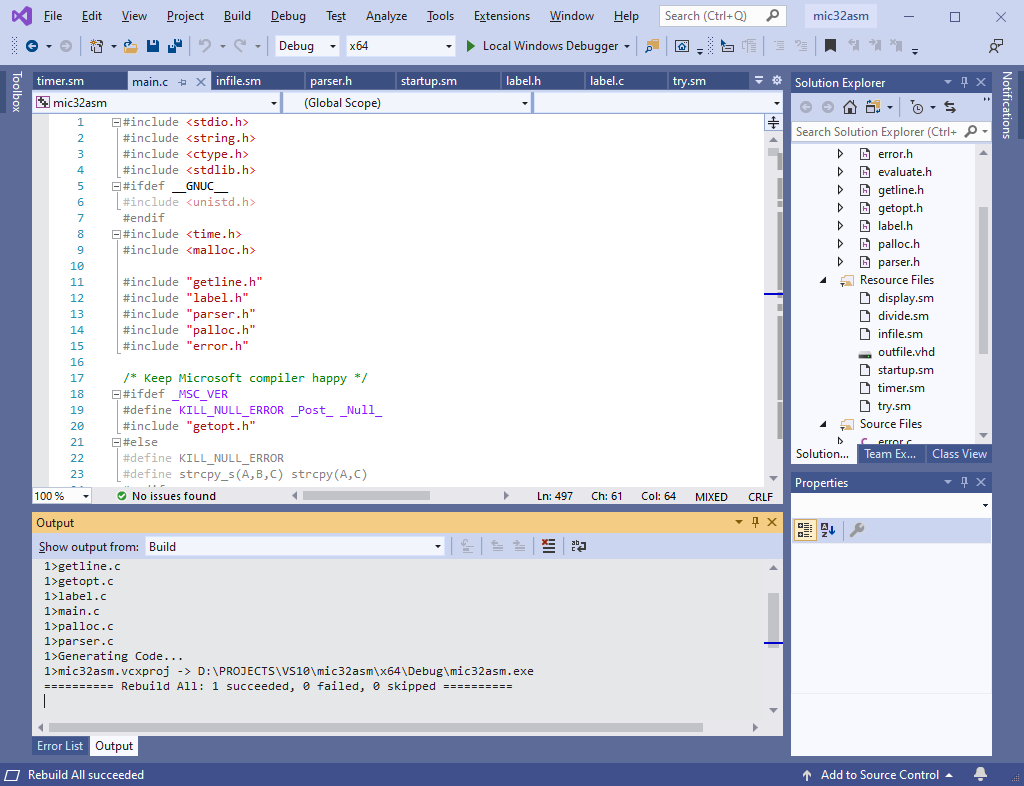
\includegraphics[width=\textwidth]{images/vs2019}
\caption{Voorbeeld van Microsoft Visual Stdio.}
\label{fig:unvs2019}
\end{figure}

We hebben nu een beeld van hoe op een computer een C-programma wordt vertaald naar instructies voor een computer. De computer kan het C-programma niet direct uitvoeren, het programma moet gecompileerd worden. Als we een wijziging in het C-programma willen doorvoeren, dan moeten we het C-programma uiteraard opnieuw compileren.

We zullen in de overige paragrafen in sneltreinvaart enkele concepten van C bespreken. In de volgende hoofdstukken wordt de taal verder uitgediept.


\section{Een minimaal C-programma}
We beginnen met het meest simpele C-programma dat mogelijk is. We willen hiermee uitleggen wat er gebeurt als dit programma gecompileerd en uitgevoerd wordt. Het programma is te zien in listing~\ref{cod:unminimaalcprogramma}. Het programma doet in feite helemaal niets, althans niet dat de gebruiker van het programma kan waarnemen. Toch gebeuren er wel degelijk dingen ``onder de motorkap''.


\begin{figure}[!ht]
\begin{lstlisting}[caption=Een minimaal C-programma.,label=cod:unminimaalcprogramma]
int main(void)
{
	return 0;
}
\end{lstlisting}
\end{figure}

Dit programma kan niet direct door de computer worden uitgevoerd, het moet eerst worden gecompileerd. Na compilatie is een \textsl{uitvoerbaar bestand}\index{uitvoerbaar bestand} beschikbaar dat wel door de computer kan worden uitgevoerd. De werking op een PC of laptop is als volgt. Als het uitvoerbare programma wordt gestart, dan zal het besturingssysteem het uitvoerbare programma in het geheugen van de computer laden. Dus ergens in het geheugen van de computer liggen de instructies die het programma vormen opgeslagen. Het besturingssysteem start het uitvoerbare programma door de processor naar de eerste instructie van het programma te leiden. Het programma (dat is het uitvoerbare programma) zal nu instructies uitvoeren. Na afloop van het programma wordt de besturing weer teruggeven aan het besturingssysteem.

Het C-programma begint met de definitie van de \textsl{functie} \texttt{main}\indextwo{main}{functie}. Een functie is een aantal instructies samengepakt onder een gemeenschappelijke noemer. \textsl{Elk C-programma heeft een functie \texttt{main}}. Tussen de haken staat het keyword \texttt{void}\indexkeyword{void}, dat aangeeft dat het uitvoerbaar programma geen gegevens meekrijgt van het besturingssysteem\footnote{Dat kan wel, zie hoofdstuk~\ref{cha:pointers}.}. Vóór \texttt{main} staat het keyword \texttt{int}\indexkeyword{int} dat aangeeft dat \texttt{main} een geheel getal teruggeeft aan het besturingssysteem.
 
Statements die in het C-programma gebruikt worden, zijn afgebakend met \textsl{accolades}\index{accolades}. Het Engelse woord hiervoor is \textsl{curly braces} of gewoon \textsl{braces}. De accolades geven het begin en einde aan van \textsl{blok}. Een blok begint met een accolade-openen (\texttt{\{}) en eindigt met een accolade-sluiten (\texttt{\}}). Over de plaats van de accolades zijn er diverse meningen. In listing~\ref{cod:unminimaalcprogramma} is de accolade-openen geplaatst onder de definitie van \texttt{main}, maar het is ook gebruikelijk om de accolade-openen te schrijven achter de definitie van \texttt{main}.
 
Binnen \texttt{main} zien we één \textsl{statement}\index{statement}. Een statement is een opdracht in de C-taal. Het statement wordt gevormd door het keyword \texttt{return}\indexkeyword{return} gevolgd door het getal 0 en een punt-komma. Bij uitvoering van dit statement wordt de waarde 0 teruggegeven aan het besturingssysteem. Dat behoeft enige uitleg. Een (gecompileerd) programma wordt gestart door het besturingssysteem. Aan het einde wordt het programma afgesloten. Het besturingssysteem ``ruimt'' het programma op en zorgt ervoor dat het gebruikte geheugen weer vrijgegeven wordt voor volgende programma's. We kunnen aan het besturingssysteem een getal teruggeven, in dit geval 0. Het is aan het besturingssysteem om hier wat mee te doen. Gebruikelijk is om 0 terug te geven als alles goed verlopen is. Een ander getal dan 0 geeft over het algemeen aan dat er iets fout gegaan is. Vanaf C99 is het niet meer nodig om dit \texttt{return}-statement uit te voeren. Dan wordt automatisch het getal 0 teruggegeven.

\section{Afdrukken op het scherm}
We kunnen het eerste programma interessanter maken door een regel tekst op het scherm af te drukken. Het programma in listing~\ref{cod:uneersteprogramma} drukt de regel \texttt{De som van 3 en 7 is 10} op het scherm af. We zullen het programma stap voor stap doorlopen.

\begin{figure}[!ht]
\begin{lstlisting}[caption=Afdrukken van de som van twee getallen.,label=cod:uneersteprogramma]
#include <stdio.h>

int main(void)
{
    int a = 3;
    int b = 7;

    int som;

    som = a + b;

	printf("De som van %d en %d is %d\n", a, b, som);

	return 0;
}
\end{lstlisting}
\end{figure}

In regel 1 wordt een zogenoemd \textsl{header-bestand}\index{header-bestand} geladen, in dit geval het bestand \texttt{stdio.h}\indextwo{stdio.h}{header-bestand}. We leggen zo meteen uit waarom dat nodig is.

In regel 3 wordt kenbaar gemaakt dat het programma de functie \texttt{main}\indextwo{main}{functie} heeft. Een C-programma heeft \textsl{altijd} de functie \texttt{main}. Het (gecompileerde) programma wordt hier gestart.

In regel 5 en 6 worden twee \textsl{variabelen}\index{variabele} gedeclareerd, de variabelen \texttt{a} en \texttt{b}. Technisch gezien is een variabele een plek in het geheugen van de computer. Een variabele kan door het programma gebruikt worden om gegevens te bewerken. Declaratie\index{declaratie} wil zeggen dat een variabele kenbaar wordt gemaakt. Bij de declaratie wordt opgegeven wat het type is van de variabele. Dit gebeurt middels het keyword \texttt{int}, dat betekent dat \texttt{a} en \texttt{b} alleen geheeltallige getallen kan opslaan (Engels: integer). Aan de variabelen worden gelijk waarden toegekend. We noemen dit \textsl{initialisatie}\index{initialisatie} van variabelen.

In regel 8 wordt de variabele \texttt{som} gedeclareerd zonder initialisatie. Dat betekent dat op dat moment de waarde (of inhoud) van de variabele \textsl{onbekend} is. Vervolgens wordt in regel 10 de som van \texttt{a} en \texttt{b} berekend middels de \textsl{optel-operator} \texttt{+}\indexop{+} en wordt het resultaat \textsl{toegekend}\index{toekenning}\indexop{=} aan variabele \texttt{som}. Vanaf regel 10 is de waarde van \texttt{som} dus 10. In regel 10 zien we zogenoemde \textsl{expressies}\index{expressie}. Zo is \texttt{a + b} een expressie en is de toekenning \mbox{\texttt{som = ...}} ook een expressie. De term expressie komt veel voor in C.

In regel 12 wordt de functie \texttt{printf}\indexfunc{printf} aangeroepen. Deze functie is al geschreven is zit in de standard library. De functie krijgt vier \textsl{argumenten}\index{argument} mee, gegevens die in de functie verwerkt worden. Het eerste argument is een \textsl{string}\index{string}. Een string is een stukje tekst, maar we spreken ook wel van een rij karakters. Daarna volgen de (waarden) van de variabelen \texttt{a}, \texttt{b} en \texttt{som}.

Het eerste argument van \texttt{printf} wordt een \textsl{format string} genoemd. Dat ligt niet in C-taal vast maar wordt algemeen gebruikt. De format string bevat karakters, zogenoemde \textsl{format specifications} en een \textsl{escape sequence}. Een format specification begint met een procentteken gevolgd door een letter. De functie \texttt{printf} gebruikt deze format specifications om de gegevens af te drukken. De eerste \texttt{\%d} zorgt ervoor dat variabele \texttt{a} wordt afgedrukt als een decimaal geheel getal. Op overeenkomstige wijze worden ook \texttt{b} en \texttt{som} afgedrukt. Aan het einde van de format string is een \textsl{escape sequence} te zien, in dit geval \texttt{\textbackslash n}. Dit zorgt ervoor dat een volgende afdruk wordt begonnen aan het begin van de volgende regel (Engels: newline).

In regel 14 wordt met het keyword \texttt{return} aangegeven dat het programma wordt afgesloten. 
Dat de return-waarde een geheel getal moet zijn, kunnen we zien aan de definitie van de functie \texttt{main}. We zien in regel 3 dat \texttt{main} een geheel getal teruggeeft (keyword \texttt{int}) en geen argumenten meekrijgt (keyword \texttt{void}).

Hoe weet de C-compiler nu hoe de functie \texttt{printf} moet worden aangeroepen? Dat wordt geregeld met een \textsl{function prototype}. We hoeven dat zelf niet op te geven want dat is al gedaan en is te vinden in het header-bestand \texttt{stdio.h}\indextwo{stdio.h}{header-bestand}. De eerste regel geeft dus aan dat dit bestand geladen moet worden. De tekens \texttt{<} en \texttt{>} geven aan dat gezocht moet worden op een bepaalde plek in het bestandssysteem. We hoeven dat verder niet te weten.

\section{Invoer van het toetsenbord}
We kunnen het vorige programma interessanter maken door aan de gebruiker te vragen om twee gehele getallen in te voeren. Naast het afdrukken van tekst met de functie \texttt{printf} maken we nu ook gebruik van de functie \texttt{scanf}\indextwo{scanf}{functie} om gehele getallen in te lezen. Het programma is te zien in listing~\ref{cod:unscanfprogramma}.

\begin{figure}[!ht]
\begin{lstlisting}[caption=Invoer van de gebruiker opvragen.,label=cod:unscanfprogramma]
#include <stdio.h>

/* Make Visual Studio happy */
#pragma warning(disable : 4996)

int main(void) 
{
    int a;
    int b;

    int som;

    printf("Geef een getal: ");
    scanf("%d", &a);

    printf("Geef nog een getal: ");
    scanf("%d", &b);

    som = a + b;

    printf("De som van %d en %d is %d\n", a, b, som);

    return 0;
}
\end{lstlisting}
\end{figure}

In regel 1 laden we weer het header-bestand \texttt{stdio.h}. Dit header-bestand is nodig om de functie-prototypes van \texttt{printf} en \texttt{scanf} te laden. In regel 4 maken we gebruik van een \textsl{pragma}\index{pragma}. Dit is een aanwijzing voor de C-compiler om iets te doen of te laten. Waarom deze pragma nodig is, kunnen we lezen in het kader op pagina~\pageref{fig:unopmerkingscanf}.

\begin{infobox}[To \texttt{scanf} or not to \texttt{scanf}...]
\label{fig:unopmerkingscanf}%
De Microsoft C-compiler bestempelt \texttt{scanf} als ``onveilig''. Een compilatie met \texttt{scanf} zal eindigen met een foutmelding. In plaats daarvan moet de functie \texttt{scanf\_s} worden gebruikt. Helaas ondersteunen andere compilers deze functie niet. Dat zal resulteren in een programma dat niet door iedere compiler kan worden vertaald. Om het probleem te omzeilen hebben we gebruik gemaakt van een \textsl{pragma}. In regel~4 geven we aan dat de C-compiler fout 4996 moet negeren. Op andere compilers, bijvoorbeeld de GNU-C compiler, wordt deze regel overgeslagen (er volgt wel een waarschuwing). Overigens wordt op vele fora gewaarschuwd voor de onveiligheid van \texttt{scanf} en worden alternatieven gegeven. Wij gebruiken \texttt{scanf} hier wel \textsl{for the sake of simplicity}. Het is beter om \texttt{scanf} te vermijden.
\end{infobox}

Het programma volgt verder de lijn van listing~\ref{cod:uneersteprogramma}. In de functie \texttt{main} declareren we drie variabelen. Daarna drukken we in regel 13 een stukje tekst of dat aangeeft wat de gebruiker moet doen. In regel 14 wordt de functie \texttt{scanf} aangeroepen die ervoor zorgt dat een geheel getal wordt ingelezen van het toetsenbord en in variabele \texttt{a} wordt gezet.

De format specification \texttt{\%d} hadden we al eerder gezien, maar de constructie \texttt{\&a} is nieuw. De ampersand (\texttt{\&}) zorgt ervoor dat aan de functie \texttt{scanf} het \textsl{adres} van variabele \texttt{a} meegegeven wordt. Het adres van de variabele is de plek waar de variabele in het geheugen ligt. Op deze manier kan \texttt{scanf} de informatie op je juiste plek zetten. In regel 17 wordt hetzelfde gedaan voor variabele \texttt{b}. We drukken voor het inlezen nog even netjes af hoe de gebruiker moet handelen. In regel 19 rekenen we de som uit van variabelen \texttt{a} en \texttt{b} en kennen dat toe aan variabele \texttt{som}. In regel 21 drukken we de drie variabelen af. Het programma wordt afgesloten in regel 23.

Als we het programma starten dan moeten we twee gehele getallen invoeren. Een mogelijke uitvoer van het programma is te zien in figuur~\ref{fig:unuitvoerprog}. De invoer van de gebruiker is vet afgedrukt.
Overigens zullen ontwikkelsystemen zoals Visual Studio aan het einde van het programma wachten tot de gebruiker op een toets drukt, anders is door de snelheid van het uitvoeren van het programma niet te zien wat is afgedrukt.

\begin{dosbox}[title=Uitvoer van het programma in listing~\ref{cod:unscanfprogramma}.,label=fig:unuitvoerprog]
Geef een getal: (*\textbf{7}*)
Geef nog een getal: (*\textbf{4}*)
De som van 7 en 4 is 11
\end{dosbox}

\section{Keywords}

In tabel~\ref{tab:unkeywords} is een lijst te zien met gereserveerde woorden. Een aantal van deze woorden hebben we algezien zoals \texttt{int}, \texttt{void} en \texttt{return}. Deze woorden worden \textsl{keywords}\index{keyword} genoemd en geven de compiler aanwijzingen over wat er moet gebeuren.

\begin{table}[!ht]
\caption{Een lijst met keywords in de C-taal.}
\label{tab:unkeywords}
\centering\ttfamily
\begin{tabular}{p{2.5cm}p{2.5cm}p{2.5cm}p{2.5cm}}
\toprule
auto &  double &  int & struct \\
break & else  & long  &  switch \\
case & enum & register & typedef \\
char & extern & return & union \\
const & float & short &  unsigned \\
continue & for & signed & void \\
default & goto & sizeof & volatile \\
do & if & static & while \\
\bottomrule
\end{tabular}
\end{table}

Een aantal van deze keywords dient als \textsl{qualifier}\index{qualifier} voor andere keywords. Zo kunnen we een variabele declareren als

\hspace*{1em}\texttt{unsigned long int a;}

Dit geeft de compiler aanwijzingen over de grootte (het aantal bits) van variabele \texttt{a}.


\section{Beslissingen}
Met behulp van de keyswords \texttt{if}\indexkeyword{if} en \texttt{else}\indexkeyword{else} kunnen in het programma beslissingen nemen op basis van een \textsl{conditie}\index{conditie}. Dit is te zien in listing~\ref{cod:unif}. We declareren twee variabelen \texttt{a} en \texttt{b} en kennen gelijk de waarden toe. In regel 8 is te zien dat getest wordt of \texttt{a} kleiner is dan \texttt{b}. We noemen het kleiner-dan-teken een \textsl{relationele operator}\index{relationele operator}. Als inderdaad blijkt dat \texttt{a} kleiner is dan \texttt{b}, dat betekent dat de conditie \texttt{a < b} waar is, worden de statements tussen de accolades in de regels 9 en 11 uitgevoerd. Is de conditie niet waar, dan worden de regels overgeslagen. Overigens mogen in dit geval de accolades weggelaten worden omdat maar één statement wordt uitgevoerd. Het is echter aan te bevelen om ze toch te gebruiken, omdat misschien later er nog statements toegevoegd worden. Een bekend voorbeeld van het niet-gebruiken van accolades is Apple's \textsl{gotofail SSL security bug}~\cite{barr2014}.

\begin{figure}[!ht]
\begin{lstlisting}[caption=Afdrukken van tekst op basis van een beslissing.,label=cod:unif]
#include <stdio.h>

int main(void)
{
    int a = 7;
    int b = 9;
    
    if (a < b)
    {
        printf("a is kleiner dan b\n");
    }
    
    return 0;
}
\end{lstlisting}
\end{figure}

Een \texttt{if}-statement kan ook gevolgd worden door een \texttt{else}-keyword en een \texttt{else}-keyword kan ook weer gevolgd worden door een \texttt{if}-keyword. In het Engels wordt dit een \textsl{multy-way branch} (to branch = vertakken) genoemd. Zie listing~\ref{cod:unifelse}.

\begin{figure}[!ht]
\begin{lstlisting}[caption=Afdrukken van tekst op basis van een beslissing.,label=cod:unifelse]
#include <stdio.h>

int main(void)
{
    int a = 7;
    int b = 9;
    
    if (a < b)
    {
        printf("a is kleiner dan b\n");
    }
    else if (a == b) 
    {
        printf("a is gelijk aan b\n");
    }
    else
    {
        printf("a is groter dan b\n");
    }
    return 0;
}
\end{lstlisting}
\end{figure}

Technisch gezien hoort de \texttt{else} in regel 16 bij de \texttt{if} in regel 12. Let erop dat het vergelijken van \texttt{a} en \texttt{b} op gelijkheid in regel 12 een \textsl{dubbele is-gelijk-teken} (\texttt{==})\indexop{==} bevat.

 
\section{Herhalingen}
Stel dat we de kwadraten van 1 t/m 10 willen afdrukken. We kunnen ervoor kiezen om tien \texttt{print}-functies aan te roepen. Maar we merken direct op dat we in feite tien keer hetzelfde moeten doen. We kunnen het afdrukken van de tien kwadraten vormgeven met een \textsl{herhaling}. Een andere, veel gebruikte term is \textsl{lus}\index{lus}. Dit is te zien in listing~\ref{cod:printkwadraten}.

We beginnen het programma met de declaratie van een aantal variabelen. Vervolgens stellen we de ondergrens, bovengrens en stapgrootte in in de regels 8 t/m 10. We willen beginnen bij de ondergrens, stoppen bij de bovengrens en bij elke herhaling nieuwe waarden afdrukken. Daarvoor gebruiken we de variabele \texttt{getal}. Zo'n variabele wordt een \textsl{lusvariabele}\index{lusvariabele} genoemd.

In regel 12 zetten we de lusvariabele op de ondergrens en gaan de lus uitvoeren. De lus wordt gekenmerkt door het keyword \texttt{while}\indexkeyword{while}. Achter het keyword \texttt{while} staat, tussen de haken, de conditie waarop de lus moet worden uitgevoerd.
Zolang de conditie \mbox{\texttt{getal <= bovengrens}} waar is, worden de statements binnen de accolades uitgevoerd. We noemen dat een \textsl{iteratie}\index{iteratie}. Is de conditie niet waar dan wordt verder gegaan met het statement die volgt op het \texttt{while}-statement.

\booklisting[]{C}{caption}{printkwadraten}{c}{!ht}

Binnen de accolades van het \texttt{while}-statement zien we drie statements. In regel 15 wordt het kwadraat berekend van de (huidige) waarde van de lusvariabele. Daarna worden de lusvariabele en het kwadraat afgedrukt. In regel 17 wordt de lusvariabele aangepast naar de nieuwe (volgende) waarde door de stapgrootte erbij op te tellen\footnote{Het is tegenwoordig in het Nederlands gebruikelijk om het Engelse woord updaten te gebruiken.}.

In geval van het kwadratenprogramma kunnen we ook een ander herhalingsstatement gebruiken: het \texttt{for}-statement. Het is een compacte schrijfwijze van het \texttt{while}-statement. We kunnen het berekenen van het kwadraat ook binnen de parameter van de functie plaatsen. Zo sparen we een variabele uit. Zie listing~\ref{cod:unfor}.

\begin{figure}[!ht]
\begin{lstlisting}[caption=Gebruik van een \texttt{for}-statement.,label=cod:unfor]
    // ...
	for (getal = ondergrens; getal <= bovengrens;
                                             getal = getal + stap)
	{
		printf("Het kwadraat van %3d is %3d\n",
                                             getal, getal*getal);
	}
    //...
\end{lstlisting}
\end{figure}


\section{Array's}
Een \textsl{array}\index{array} is een lijst variabelen onder een gemeenschappelijke noemer. Zo declareren we vijf floating point-getallen (getallen met een komma)\index{floating point} met

\hspace*{1em}\texttt{double lijst[5];}\indexkeyword{double}

en kunnen we gebruik maken van de variabelen

\hspace*{1em}\texttt{lijst[0] lijst[1] lijst[2] lijst[3] lijst[4]}

Tussen de blokhaken \texttt{[]}\indexop{[]} staat het \textsl{elementnummer} en de variabelen worden de \textsl{elementen} van de array genoemd. In listing~\ref{cod:arraygemiddelde} is een programma te zien met een array.

\booklisting[]{C}{Gemiddelde van vijf getallen}{arraygemiddelde}{c}{!ht}

De array mag bij declaratie gelijk geïnitialiseerd worden zoals te zien is in regel 5\footnote{We hebben als getallen vijf wiskundige constanten genomen. De lezer wordt uitgedaagd uit te zoeken welke constanten dat zijn.}. We berekenen van deze vijf elementen de gemiddelde waarde. We doen dat door eerst de som van de vijf element te berekenen en vervolgens te delen door 5. Met behulp van een \texttt{for}-statement wordt ``langs de array gelopen''; bij elke iteratie selecteren we een element en tellen dat op bij de som van de tot dan toe gesommeerde elementen. De regel

\hspace*{1em}\texttt{som = som + lijst[index];}

selecteert dus een element uit de array en telt dat op bij de som. In regel 13 drukken we het gemiddelde af door de som te delen door 5. We hoeven daarvoor niet een aparte variabele te declareren, we kunnen als argument gewoon \texttt{som / 5.0} gebruiken.


\section{Functies}
C biedt een handige manier om een groep statement, bijvoorbeeld berekeningen, onder te brengen in een \textsl{functie}\index{functie}. Als de functie eenmaal geschreven is hoeven we ons niet druk te maken over hoe de de berekeningen worden gedaan, we moeten alleen maar weten hoe we de functie moeten gebruiken. We hebben al drie functies gezien: \texttt{printf}, \texttt{scanf} en \texttt{main}. De functies \texttt{printf} en \texttt{scanf} zijn al beschikbaar via de standard library. We hoeven niet te weten hoe de functies werken, alleen maar hoe ze moeten worden aangeroepen.

Laten we eens de wortels bepalen van de getallen 0 t/m 10. Daartoe schrijven we een functie \texttt{sqrt\_babylonian} die de wortel van een getal bepaalt volgens de Babylonische methode. Dit is een iteratieve methode om de wortel van een getal steeds nauwkeuriger te benaderen. De manier waarop dat gebeurt is te zien in vergelijking~\eqref{equ:sqrtbab}.
%
\begin{equation}
\label{equ:sqrtbab}
\begin{split}
x_0 &= S &&&& \text{beginsituatie} \\
x_{n+1} &= \dfrac{1}{2}\cdot\left(x_n + \dfrac{S}{x_n}\right) &&&& \text{nieuwe situatie}\\
\sqrt{S} &= \lim_{n\rightarrow\infty} x_n &&&& \text{uiteindelijke resultaat}
\end{split}
\end{equation}
%
We lezen dit als volgt. We beginnen met het getal $S$ waarvan we de wortel willen berekenen ($x_0= S$). De tweede, iteratieve stap, is het berekenen van de volgende benadering. We berekenen dat met de middelste vergelijking uit~\eqref{equ:sqrtbab}. De laatste stap geeft aan dat als we de wortel willen bepalen, de tweede stap oneindig vaak herhaald moet worden. Natuurlijk is dat niet realiseerbaar. We kunnen maar een eindig aantal stappen uitrekenen. Het blijkt dat voor de wortel slechts tien stappen nodig zijn om de wortel redelijk te benaderen.

De functie is te zien in listing~\ref{cod:sqrt_babylonian}. We maken hier gebruik van het datatype \texttt{double}\indexkeyword{double}, een floating point-datatype met een nauwkeurigheid van ongeveer 16 decimale cijfers. Zowel het argument als het returnwaarde is van dit datatype. We beginnen met de functiedefinitie

\hspace*{1em}\texttt{double square\_root(double s)}

Binnen de functie maken we gebruik van de twee variabelen \texttt{xiter} en \texttt{i}. \texttt{xiter} wordt gebruikt om de nieuwe waarde van de wortel te berekenen en \texttt{i} wordt gebruik om het aantal iteraties bij te houden.
We testen in regels 8 t/m 10 of het argument 0 is en geven dan direct de waarde 0 terug.

\booklisting[]{C}{Programma om de wortels van 1 t/m 10 af te drukken}{sqrt_babylonian}{c}{!ht}

In het \texttt{for}-statement worden tien iteraties van de middelste formule uit~\eqref{equ:sqrtbab} uitgevoerd. Bij elke iteratie wordt de waarde van de wortel steeds beter benaderd. Als het \texttt{for}-statement klaar is, wordt deze waarde via \texttt{return} teruggegeven aan de aanroeper. In \texttt{main} worden met behulp van een \texttt{for}-statement de wortels van 0 t/m 10 berekend en afgedrukt.

Overigens bevat de \textsl{mathematical library} een implementatie van de wortel-functie. We hoeven dat niet zelf te schrijven.


\section{Codeerstijlen}
C is erg coulant in het vormgeven van een programma. Het maakt meestal niet uit waar we de statements zetten en hoe een groep statements worden afgebakend. We kunnen regels overslaan (een lege regel) en we kunnen statements vooraf laten gaan door een willekeurig aantal spaties of we kunnen instructies achter elkaar op een regel plaatsen.

Een mooi voorbeeld van hoe onze wortelfunctie onleesbaar te maken is, kunnen we zien in listing~\ref{cod:sqrt_babylonian_bad_style}. De functie wordt door de C-compiler correct vertaald maar is voor een mens slecht leesbaar. De code in listing~\ref{cod:sqrt_babylonian} is veel beter leesbaar.

\booklisting[]{C}{Een functie om een wortel van een getal te bepalen}{sqrt_babylonian_bad_style}{c}{!ht}

Hoe een programma uiterlijk wordt vormgegeven noemen we een \textsl{codeerstijl}\index{codeerstijl}. Er zijn behoorlijk wat stijlen maar we zullen er twee noemen.

In de K\&R-stijl (Kernighan en Ritchie)\index{K\&R-stijl} wordt de accolade-openen \textsl{achter} een functie, beslis-sings- of herhalingstatement geschreven. De statements hierbinnen worden \textsl{ingesprongen} (dat wordt in het Engels \textsl{indentation} genoemd)\index{inspringen!van code}\index{indentation}. Bij gebruik van in elkaar verweven beslissings- of herhalingstatement worden de statements verder of dieper ingesprongen.

\begin{lstlisting}[caption=K\&R-stijl.]
if (a < b) {
    (*\normalfont\textsl{statements}*)
}
\end{lstlisting}

In de Allman-stijl\index{Allman-stijl} wordt de accolade-openen \textsl{onder} een functie, beslissings- of herhalingstatement geschreven. De statement hierbinnen worden \textsl{ingesprongen}. Bij gebruik van in elkaar verweven beslissings- of herhalingstatement worden de statement verder of dieper ingesprongen.

\begin{lstlisting}[caption=Allman-stijl.]
if (a < b)
{
    (*\normalfont\textsl{statements}*)
}
\end{lstlisting}

\section{En verder...}
We hebben nu enkele concepten van C uitgelegd. Maar de taal kan meer. Wat we niet behandeld hebben zijn \textsl{pointers}, \textsl{structures} en \textsl{bestandsverwerking}. Deze concepten zullen in de volgende hoofdstukken worden uitgelegd.
